\documentclass{article}
\usepackage[utf8]{inputenc}
\usepackage[portuguese]{babel}
\usepackage[T1]{fontenc}
\usepackage{natbib}
\usepackage[toc,page]{appendix}
\usepackage{graphicx}
\usepackage{amsmath}
\usepackage{algorithm2e}
\usepackage[procnames]{listings}
\usepackage{color}

\title{???}
\author{Marco Lúcio de Carvalho Júnior}
\date{31 de Agosto de 2017}

\begin{document}
    \maketitle

    \newpage

    \abstract

        Em diversas áreas das ciências, existem informações apresentadas em inúmeros formatos e diferentes escalas.
        A primeira vista, alguns desses dados podem ser interpretados de forma confusa.
        Felizmente, é possível representar conhecimentos dispostos em alta dimensão para representações em baixa dimensão.
        Dessa forma, essas mesmas informações podem ser dispostas de forma organizada.
        Nesse projeto de pesquisa, o método utilizado para exemplificar essa situação se chama Diffusion Map.
        Conceitos como distância euclidiana, normalização de dados, matrizes diagonais e transpostas serão abordados.
        Ademais, autovalores e autovetores, k-means e medidas da teoria da informação, como pureza e informação mútua, serão necessários para uma compreensão apurada da origem do projeto até o resultado final.
        Ao fim da implementação do algoritmo, a avaliação de agrupamento NMI (normalized mutual information) foi operada com a finalidade de ser responsável pela validação dos resultados.
        A partir dessa avaliação, foi concluído que o resultado do projeto possui níveis satisfatórios de aceitação. \\

        \\ Palavras chaves: diffusion map, redução de dimensionalidade, k-means, NMI. \\

        In several areas of science, information is presented in numerous formats and different scales.
        At first sight, some of the data can be interpreted in a confusing way.
        Fortunately, it's possible to represent knowledge arranged in high dimensions for representations in a small dimension.
        In this way, the same information can be arranged in an organized way.
        In this research project, the method used to exemplify this situation is called Diffusion Map.
        Concepts such as Euclidean distance, data normalization, diagonal and transposed matrices will be addressed.
        In addition, eigenvalues and eigenvectors, k-means and measures of information theory, such as purity and mutual information, will be necessary for an accurate understanding of the origin of the project to the final result.
        At the end of the implementation of the algorithm, the NMI (normalized mutual information) grouping was performed in order to be responsible for the validation of the results.
        From this evaluation, it was concluded that the project result has satisfactory levels of acceptance. \\

        \\ Keywords: diffusion map, dimensionality reduction, k-means, NMI.

    \newpage

    \tableofcontents

    \newpage

    \section{Introdução}

        O Diffusion Map pode ser descrito como um framework de redução de dimensionalidade ou de extração de funcionalidade \cite{coifman2006diffusion}, e é usado para a organização geométrica estrutural multi-escala de gráficos e subconjuntos do $\rm I\!R^{n}$\cite{coifman2005geometric}.
        O primeiro é o processo de reduzir um número de variáveis aleatórias em um dataset.
        Pode ser aplicado para facilidade na visualização de dados, otimização do desempenho em alguns modelos de aprendizagem de máquina e, consequentemente, deixa de ser uma necessidade possuir grandes espaços de armazenamento.
        O segundo pode ser explicado como a criação de valores com propósitos informativos, a partir de um dataset, e utilizados para interpretações apuradas.
        De certa forma, envolve em reduzir a quantidade de recursos necessários para se ter uma completa descrição de uma massa de dados, ainda mantendo a precisão necessária.

    \section{Objetivo}

        O projeto de pesquisa tem como objetivo testar o efeito da redução de dimensionalidade sobre agrupamentos, em termos de qualidade e de tempo.

    \section{Material e Métodos}

        A linguagem de programação utilizada para o projeto foi R\cite{R}.
        Ela foi escolhida devido aos diversos métodos e pacotes nativos da linguagem.
        Para facilitar o desenvolvimento na linguagem, o RStudio Desktop, ambiente integrado de desenvolvimento (IDE) mais popular da linguagem, foi escolhido para se gerar os resultados.

        Para realizar a implementação do algoritmo Diffusion Map, é necessário descrever conceitos relativos ao framework e seguir alguns passos.

        \subsection{Diffusion Map}

            Utilizando uma matriz $X$ gerada aleatoriamente, com 4 propriedades e 20 amostras, deve-se:

            \begin{center}
                \begin{tabular}{llll}
                    V1         & V2         & V3         & V4           \\
                    \hline
                    4.3 & 5.89 & 5.53 & 5.99 \\
                    3.55 & 2.37 & 2.65 & 1.35 \\
                    5.68 & 1.19 & 4.08 & 3.7 \\
                    4.61 & 3.74 & 2.51 & 3.27 \\
                    5.83 & 2.92 & 2.98 & 5.81 \\
                    2.89 & 5.03 & 3.09 & 6.64 \\
                    5.55 & 2.3 & 6.12 & 4.58 \\
                    4.07 & 3.34 & 6.85 & 5.14 \\
                    2.95 & 2.77 & 6.51 & 4.36 \\
                    5.2 & 2.33 & 6.14 & 6.46 \\
                    4.56 & 2.17 & 4.05 & 5.49 \\
                    3.44 & 6.86 & 1.41 & 5.89 \\
                    1.15 & 6.64 & 5.68 & 1.42 \\
                    4.01 & 2.22 & 1.46 & 1.76 \\
                    4.89 & 2.62 & 1.69 & 4.24 \\
                    2.4 & 2.11 & 3.28 & 6.29 \\
                    2.31 & 4.63 & 3.67 & 1.24 \\
                    3.01 & 2.08 & 6.35 & 3.86 \\
                    4.45 & 1.75 & 1.19 & 6.2 \\
                    4.53 & 2.59 & 6.22 & 1.65
                \end{tabular}
            \end{center}

            \begin{enumerate}

                \item Normalizar cada coluna da matriz $X$ em uma matriz temporária $T1$:
                    \[
                        T1=\frac{X-min(X)}{max(X)-min(X)}
                    \]

                    \begin{center}
                        \begin{tabular}{llll}
                            V1         & V2         & V3         & V4        \\
                            \hline
                            0.6730769 & 0.82892416 & 0.76678445 & 0.87962963 \\
                            0.5128205 & 0.20811287 & 0.25795053 & 0.02037037 \\
                            0.9679487 & 0.00000000 & 0.51060071 & 0.45555556 \\
                            0.7393162 & 0.44973545 & 0.23321555 & 0.37592593 \\
                            1.0000000 & 0.30511464 & 0.31625442 & 0.84629630 \\
                            0.3717949 & 0.67724868 & 0.33568905 & 1.00000000 \\
                            0.9401709 & 0.19576720 & 0.87102473 & 0.61851852 \\
                            0.6239316 & 0.37918871 & 1.00000000 & 0.72222222 \\
                            0.3846154 & 0.27865961 & 0.93992933 & 0.57777778 \\
                            0.8653846 & 0.20105820 & 0.87455830 & 0.96666667 \\
                            0.7286325 & 0.17283951 & 0.50530035 & 0.78703704 \\
                            0.4893162 & 1.00000000 & 0.03886926 & 0.86111111 \\
                            0.0000000 & 0.96119929 & 0.79328622 & 0.03333333 \\
                            0.6111111 & 0.18165785 & 0.04770318 & 0.09629630 \\
                            0.7991453 & 0.25220459 & 0.08833922 & 0.55555556 \\
                            0.2670940 & 0.16225750 & 0.36925795 & 0.93518519 \\
                            0.2478632 & 0.60670194 & 0.43816254 & 0.00000000 \\
                            0.3974359 & 0.15696649 & 0.91166078 & 0.48518519 \\
                            0.7051282 & 0.09876543 & 0.00000000 & 0.91851852 \\
                            0.7222222 & 0.24691358 & 0.88869258 & 0.07592593
                        \end{tabular}\par
                        Matriz $T1$, ou matriz $X$ normalizada.
                    \end{center}

                \item Calcular a distância euclidiana da matriz temporária $T1$ em uma outra matriz temporária $T2$:

                    \begin{center}
                        \begin{tabular}{llll}
                            1         & 2          & \dots      & 19         \\
                            \hline
                            0         & 1.1867296  & \dots      & 1.0009759  \\
                            1.1867296 & 0          & \dots      & 0.6680393  \\
                            1.0097196 & 0.7096978  & \dots      & 0.6390774  \\
                            0.8286042 & 0.4865320  & \dots      & 0.7490521  \\
                            \vdots    & \vdots     & \vdots     & \vdots     \\
                            1.0009759 & 0.6680393  & \dots      & 0
                        \end{tabular}\par
                        Matriz $T2$, ou a distância euclidiana da matriz $T1$.
                    \end{center}

                    A expressão para o cálculo da mesma pode ser intepretada como $d_{ij}=x_{i}-x_{j}$, onde $T2$ é simétrica ($x_{ij}=x_{ji}$).

                \item Computar a matriz diagonal $D$:
                \[
                    D_{i,j}=\sum_{j}X_{i,j}
                \]

                \item Normalizar a matriz resultante $X$ utilizando o parâmetro $a$ com um valor experimental de $0.5$:
                \[
                    X^{(a)}=D^{-a}XD^{-a}
                \]

                \item Determinar a matriz normalizada $M$:
                \[
                    M=(D^{(a)})^{-1}X^{(a)}
                \]

            \end{enumerate}

            Utilizando a transposta da matriz $M$, deve-se inferir os autovalores e autovetores, sendo o último utilizado como as coordenadas para os dados.
            O Diffusion Map pode ser definido através da seguinte expressão:
            \[
                \Psi_{t}(x)=(\lambda_{1}^{t}\psi_{1}(x),\lambda_{2}^{t}\psi_{2}(x),\dots,\lambda_{k}^{t}\psi_{k}(x))
            \]

            \begin{center}
                \begin{tabular}{llll}
                    V1         & V2         & V3         \\
                    \hline
                    -0.165383117600583 & -0.044930797721958 & -0.320482245008518 \\
                    0.281021999543499 & 0.260115295064566 & 0.198404624672686 \\
                    0.00431332509469606 & -0.111259806626831 & 0.370392589636153 \\
                    0.264946824706613 & -0.00696921144708202 & 0.107404964279494 \\
                    0.0590245213128726 & -0.343382022781831 & 0.0727510036496673 \\
                    0.0408952706510422 & -0.134195531344165 & -0.440176457597071 \\
                    -0.273987309951723 & -0.0784384907558747 & 0.232334550169892 \\
                    -0.371551526336149 & 0.0336823995759296 & -0.0184267548456168 \\
                    -0.315833871549398 & 0.172067056262753 & -0.00685892361084542 \\
                    -0.305653275104874 & -0.198359164548154 & 0.0513521211743266 \\
                    -0.0838709464153498 & -0.270949082895018 & 0.11981312303777 \\
                    0.187532533713911 & -0.0614746759869924 & -0.447709060207091 \\
                    0.0352220231162394 & 0.417156381795881 & -0.274401802132031 \\
                    0.355564505156357 & 0.147006284902527 & 0.194501345982239 \\
                    0.28691040587153 & -0.195855664484792 & 0.136787414600362 \\
                    0.00419067840165033 & -0.148884056859812 & -0.18740933291274 \\
                    0.176343737565095 & 0.396308772585093 & -0.0870727864082156 \\
                    -0.277470813207977 & 0.194773853044889 & 0.083166623223684 \\
                    0.202085232910111 & -0.310727814897057 & -0.0218855133688297 \\
                    -0.104300197877563 & 0.28431627711793 & 0.237514515664684
                \end{tabular}\par
                Matriz de autovetores formada a partir da matriz $X$.
            \end{center}

        \subsection{K-means e NMI}

            Para que os resultados sejam validados, é necessário utilizar o método de quantização vetorial k-means para extrair os agrupamentos das coordenadas de dimensão $n$, bem como definir o número $k$ de agrupamentos.

            Após isso, é preciso definir a informação mútua $I$ e a entropia $H$.
            A primeira mede a quantidade de informação que a presença/ausência de um termo contribui para a decisão correta de classificação,
            A segunda usa um conjunto de dados como entrada e calcula a entropia de acordo com o método de estimador de entropia.
            Utilizando ambos, deve-se calcular o NMI através da expressão a seguir:
            \[
                \text{NMI}(x,y)=\frac{I(x,y)}{[H(x)+H(y)]/2}
            \]

            Para validar a implementação e eficácia do método utilizado, o NMI deve ser comparado com o valor de pureza.
            Os agrupamentos defeituosos têm valores de pureza próximos de 0, enquanto que um agrupamento perfeito tem uma pureza de 1.

    \section{Discussões e Resultados}

        O dataset multivariante de flores Iris\cite{fisher1936use} foi utilizado como objeto de entrada para esse método.
        Adicionalmente, foi utilizado um dataset formado por características de corpos celestes, como coordenadas e informações relacionadas ao brilho.

        Utilizando os datasets supracitados durante a implementação, os autovetores gerados foram utilizados para plotagem (ver Figura 1 e Figura 2).

        \begin{itemize}
            \item\textit{range} e \textit{diff} para normalização das colunas da matriz;
            \item\textit{colSums} e \textit{diag} para a matriz ser computada diagonalmente;
            \item\textit{\%*\%} para multiplicação das matrizes;
            \item\textit{solve} para o cálculo da matriz inversa;
            \item\textit{t} para descobrir a matriz transposta;
            \item\textit{eigen} para identificação da lista dos autovalores e autovetores
        \end{itemize}

        \begin{figure}
            \begin{center}
                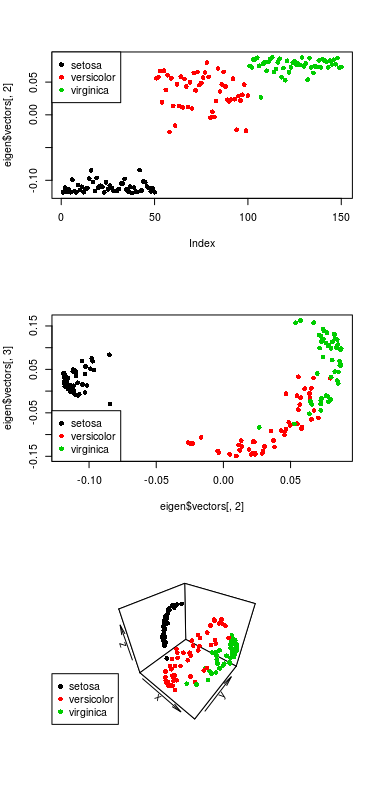
\includegraphics[width=0.8\textwidth,height=0.4\textheight]{iris.png}
            \end{center}
            \caption{Dataset Iris nos espaços $\rm I\!R^{1}$, $\rm I\!R^{2}$ e $\rm I\!R^{3}$}
        \end{figure}

        \begin{center}
            \begin{tabular}{llll}
                V2         & V3         & V4         \\
                \hline
                -0.118308705863513 & 0.0320599573859793 & 0.0394710633497636 \\
                -0.11126752124219 & -0.00521000250709525 & -0.0662543875711374 \\
                -0.118040543325841 & 0.0108438086999693 & -0.0505667766093304 \\
                -0.114081547299355 & 0.0006152854119494 & -0.0722843220130793 \\
                -0.118288411135076 & 0.0386602653432783 & 0.0445189451934104 \\
                -0.0990674751135123 & 0.0514155298114675 & 0.109811730137344 \\
                -0.116538081194761 & 0.0195407400374584 & -0.0206121860568938 \\
                -0.118550146248947 & 0.0223359897165494 & 0.0155434574563725 \\
                -0.107350970039746 & -0.00729743478136912 & -0.109398348648671 \\
                -0.114872674541133 & 0.00368895107309619 & -0.0505154444440465 \\
                -0.109919504644431 & 0.0457965833181171 & 0.0863785207235528 \\
                -0.11816115548344 & 0.0198372454238986 & -0.00225437451007698 \\
                \vdots & \vdots & \vdots \\
                0.0731014913754329 & -0.0161795165632858 & 0.0270602743904985
            \end{tabular}\par
            Matriz de autovetores formada a partir do dataset Iris.
        \end{center}

        \begin{center}
            \begin{tabular}{llll}
                Informação mútua & Entropia & NMI \\
                \hline
                0.7548233 & 1.058582 & 0.7130512 \\
                0.7817411 & 1.093183 & 0.7151056 \\
                0.884799 & 1.087215 & 0.8138214
            \end{tabular}\par
            Medidas da teoria da informação utilizadas nos espaços $\rm I\!R^{1}$, $\rm I\!R^{2}$ e $\rm I\!R^{3}$, respectivamente.
        \end{center}

        \begin{figure}
            \begin{center}
                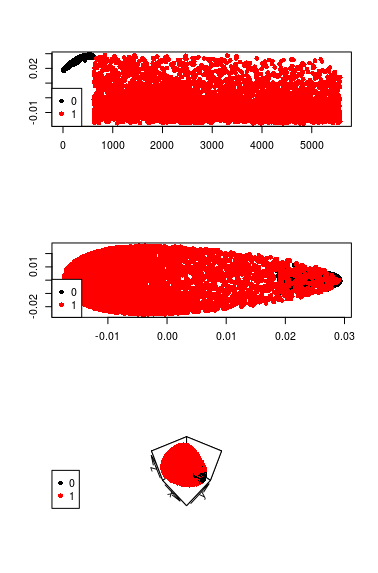
\includegraphics[width=0.8\textwidth,height=0.4\textheight]{stars.png}
            \end{center}
            \caption{Uma das centenas de plotagens dos datasets de estrelas nos espaços $\rm I\!R^{1}$, $\rm I\!R^{2}$ e $\rm I\!R^{3}$}
        \end{figure}

        \begin{center}
            \begin{tabular}{llll}
                V2         & V3         & V4         \\
                \hline
                -0.0211278753010298 & -0.00330919104764449 & 0.00141203051584593 \\
                -0.021434348994958 & -0.00172939515245416 & -0.0012855562258613 \\
                -0.0214099631831477 & 0.00217388035710803 & 0.0012824873846322 \\
                -0.0204719559303992 & -0.00860116834543878 & 0.00322173319387549 \\
                -0.0215668012786429 & -0.00145352575061309 & -0.000829634021347016 \\
                -0.0212510774054967 & 0.00436560220625638 & -0.000501455799458068 \\
                -0.021122783960784 & -0.0022866276590285 & 0.00574657919959098 \\
                -0.0215962935402548 & -0.00130613970407803 & 0.00124212369585348 \\
                -0.0210981383803671 & -0.00479598243132328 & -0.0030736131928845 \\
                -0.0210603375685055 & -0.00603910965000538 & 0.0018805414179854 \\
                -0.0216976746844701 & -0.00179873113752453 & -0.00302157180179202 \\
                -0.0212848633817281 & -0.00182118324179929 & -0.00533304170370278 \\
                \vdots & \vdots & \vdots \\
                -0.0147965033764924 & -0.0152972356294561 & -0.00476002514237425
            \end{tabular}\par
            Matriz de autovetores formada a partir de uma das centenas de datasets de estrelas.
        \end{center}

        \begin{center}
            \begin{tabular}{llll}
                Informação mútua & Entropia & NMI \\
                \hline
                0.0005217854 & 0.4154301 & 0.001256013 \\
                0.006922954  & 0.4152497 & 0.01667179  \\
                0.006657727  & 0.4141846 & 0.0160743
            \end{tabular}\par
            Medidas da teoria da informação utilizadas nos espaços $\rm I\!R^{1}$, $\rm I\!R^{2}$ e $\rm I\!R^{3}$, respectivamente.
        \end{center}

        \newpage

    \section{Conclusões}

        Com as medidas relativas a teoria da informação apontando para níveis satisfatórios, é possível afirmar que o projeto de pesquisa obteve resultados satisfatórios.
        É encorajado a utilização em outros datasets e matrizes para descoberta de novos resultados.
        Deve-se também verificar a utilização do método hungaro, para resolução de problemas de otimização.

    \bibliographystyle{ieeetr}
    \bibliography{references}
\end{document}